\documentclass[11pt,letterpaper]{article}
\usepackage[lmargin=1in,rmargin=1in,bmargin=1in,tmargin=1in]{geometry}
\usepackage{checkins}

\pgfplotsset{soldot/.style={color=black,only marks,mark=*},
		holdot/.style={color=black,fill=white,only marks,mark=*},
		compat=1.12
}

% -------------------
% Content
% -------------------
\begin{document}
\thispagestyle{title}

% 01/15
\checkin{01/15} \textit{True/False}: If $f(3)= 5$, then $\ds\lim_{x \to 3} f(x)= 5$. \pspace

\sol The statement is \textit{false}. Recall that the limit of a function (if it exists) is what the output gets `close' to as the input gets `close' to its limiting value. The fact that $f(3)= 5$ does not mean the outputs are all `close' to 5 when $x$ is `close' to 3. For instance, consider the function $f(x)$ plotted below.
	\[
	\fbox{%
	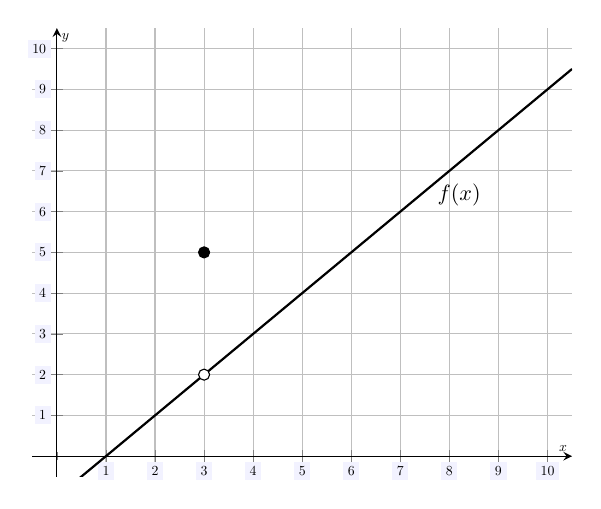
\begin{tikzpicture}[scale=1,every node/.style={scale=0.5}]
	\begin{axis}[
	grid=both,
	axis lines=middle,
	ticklabel style={fill=blue!5!white},
	xmin= -0.5, xmax=10.5,
	ymin= -0.5, ymax=10.5,
	xtick={-1,0,...,11},
	ytick={-1,0,...,11},
	minor tick = {-11,-10,...,11},
	xlabel=\(x\),ylabel=\(y\),
	samples=20]
	\node at (8.2,6.4) {\scalebox{1.6}{$f(x)$}};
	\addplot[thick, samples=5, domain= -0.5:10.5] {x - 1};
	\addplot[soldot] coordinates{(3,5)};
	\addplot[holdot] coordinates{(3,2)};
	\end{axis}
	\end{tikzpicture}
	}
	\]
Despite the fact that $f(3)= 5$, $\ds\lim_{x \to 3} f(x)= 2$ because all the outputs are `close' to 2 when the inputs are `close' to 3. \pvspace{1.3cm}



% 01/17
\checkin{01/17} \textit{True/False}: Let $f(x)$ be a function defined on all real numbers such that $\ds\lim_{x \to \pi} f(x)= 10$. Then it must be that $\ds\lim_{x \to \pi^+} f(x)= 10$. \pspace

\sol The statement is \textit{true}. Recall that the limit (if it exists) is what the output gets `close' to as the input gets `close' to its limiting value. Because $\ds\lim_{x \to \pi} f(x)= 10$, the outputs of $f(x)$ are all `close' to 10 whenever $x$ is `close' to $\pi$---no matter how $x$ is `close' to $\pi$. The right-hand limit $\ds\lim_{x \to \pi^+} f(x)$ asks what the outputs are `close' to if $x$ is `close' to $\pi$---but bigger than $\pi$. But we already know that the outputs are `close' to 10. Therefore, it must be that $\ds\lim_{x \to \pi^+} f(x)= 10$. Recall that $\ds\lim_{x \to a} f(x)= L$ if and only if $\lim_{x \to a^-} f(x)= L$ and $\lim_{x \to a^+} f(x)= L$. \pvspace{1.3cm}



% 01/22
\checkin{01/22} $\ds\lim_{x \to \infty} \left(1 + \dfrac{1}{3x} \right)^x= e^3$ \pspace

\sol The statement is \textit{false}. Recall that $\ds\lim_{x \to \infty} \left(1 + \dfrac{1}{x} \right)^x= e$. But then\dots
	\[
	\lim_{x \to \infty} \left(1 + \dfrac{1}{3x} \right)^x= \lim_{x \to \infty} \left(1 + \dfrac{1}{3x} \right)^{x \cdot 3/3}= \lim_{x \to \infty} \left[ \left(1 + \dfrac{1}{3x} \right)^{3x} \right]^{1/3}= e^{1/3}= \sqrt[3]{e}
	\] \pvspace{1.3cm}



% 01/24
\checkin{01/24} $\ds\lim_{x \to \infty} \left(1 + \dfrac{1}{x} \right)^x= \left(1 + 0\right)^\infty= 1^\infty= 1$ \pspace

\sol The statement is \textit{false}. One does obtain $1^\infty$ after na\"ively plugging in $x= \infty$. However, $\infty$ is not a number; moreover, although one might feel otherwise, it is simply need not be the case that $1^\infty= 1$. Indeed, $1^\infty$ is an indeterminant form. One could correctly recall that\dots
	\[
	\lim_{x \to \infty} \left(1 + \dfrac{1}{x} \right)^x= e
	\] \pvspace{1.3cm}




















\end{document}